\clearpage
\section{Close proximity detection}

During the autonomous navigation the rover will be using 4 ultrasonic sensors for close proximity detection. These sensors will be placed on each of the four sides of the rover, at the same height as the wheels to help detect objects within a close distance of the rover.

\begin{figure}[H]
	\centering
	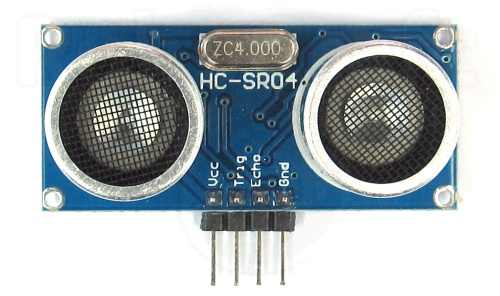
\includegraphics[width=.3\linewidth]{images/hcsr40.jpg}
	\caption{The specific ultrasonic sensors are 4 \textbf{HC-SR04}.}
\end{figure}


To avoid damaging the Raspberry pi  when using these ultrasonic sensor a voltage divider is needed in order to protect the input pins on the Raspberry pi. Since the ultrasonic sensor operates at 5V, the output will be 5V. The GPIO ports on the Raspberry Pi operate at 3.3V, so the voltage divider is used to limit the voltage going into the input port, while still providing a correct signal.
When the sensors are initially powered on they require a few milliseconds to initialize, before they can be used to take measurements. This is recommended in the datasheet.

The HC-SR04 operates using 4 pins: Vcc, Trigger, Echo, Gnd.
The trigger pin on the sensor is connected to a GPIO-OUT and the echo pin is connected to a GPIO-IN.

\begin{figure}[H]
	\centering
	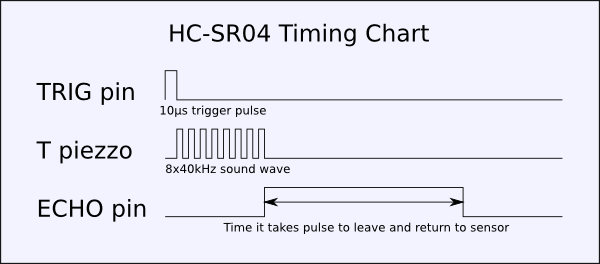
\includegraphics[width=.5\linewidth]{images/hcsr04timingchart.png}
	\caption{The HC-SR04 timing chart\cite{hcsr04timingchart}}
\end{figure}

A 10us pulse is sent from the sensor using the trigger pin, the echo pin receives a HIGH-pulse equivalent to how long it took to hear the echo. This means that length of this high-pulse is proportional to how far away the object is that distance is being measured between.\cite{ultrasonichowitworks}

$distance = \frac{(stoptime-startime) * 34000}{2}$

The above calculation is done using the speed of sound which is $speed = 340m/s$, which in centimetres is $34000cm/s$.

\clearpage
\lstinputlisting[firstline=14, lastline=32, title=ultrasonic.py, language=Python]{../code/ultrasonic-module/ultrasonic.py}

The snippet of code above is the function that gets the distance between the ultrasonic sensor module and the current object in front of it.
On line 3 the trigger output is set to High for 10us to create the ultrasonic burst. When the burst returns the input pin ECHO goes high for the duration of the pulse, which is measured by the subtracting the stop time from the start time.
The distance is returned in centimetres, since the speed of sound ($340m/s$) has been converted to centimetres per second.